\documentclass[a4paper]{article}
\usepackage[utf8]{inputenc}
\usepackage[russian]{babel}
\usepackage{listings}
\usepackage[a4paper]{geometry}
\usepackage{indentfirst}
\usepackage{graphicx}
\usepackage{caption}
\usepackage{float}
\usepackage{amssymb}
\usepackage{physics}
\usepackage{subfig}

\begin{document}

\title{Лабораторная работа 7 по курсу <<Вычислительные задачи прикладной математики>>. \\Отчёт.}
\author{Владислав Соврасов\\ 2-о-051318}
\date{}
\maketitle

\section{Сравнение наивного и Gillespie методов для моделирования процесса случайного распада вещества}

В первой части работы рассматривается уравнение \(\dot x = -x, x(0)=x_0\), описывающее
поведение среднего количества молекул в процессе распада вещества. Это уравнение было
смоделировано с помощью наивного алгоритма, алгоритма Gillespie а также решено
методом Рунге-Кутты 4го порядка. Полученные численные решения представлены на
рис. \ref{fig:1d_decay}. Видно, что две стохастические реализации процесса распада отличаются
от детерминированного решения и друг от друга. В наивном алгоритме \(\Delta t=0.01/a(0)\), что
обеспечивает для данного уравнения выполнение требования \(\Delta t \ll 1/a(x)\) в течение всего процесса решения.
График решения, полученного наивным алгоритмом, имеет характерные стуепньки, которые означают выполнение
нескольких итераций подряд без уменьшения количества молекул. Алгоритм Gillespie совершает итерации
только в моменты распада, что позволяет ему работать на порядок быстрее (см. табл. \ref{tab:time}).

\begin{table}[h!]
  \centering
  \begin{tabular}{ c|c }
     Метод & Время, с  \\
     \hline
     Naive & 0.0257  \\
     Gillespie & 0.0031
  \end{tabular}
\caption{Время выполнения различных методов}
\label{tab:time}
\end{table}


\begin{figure}[H]
  \center
  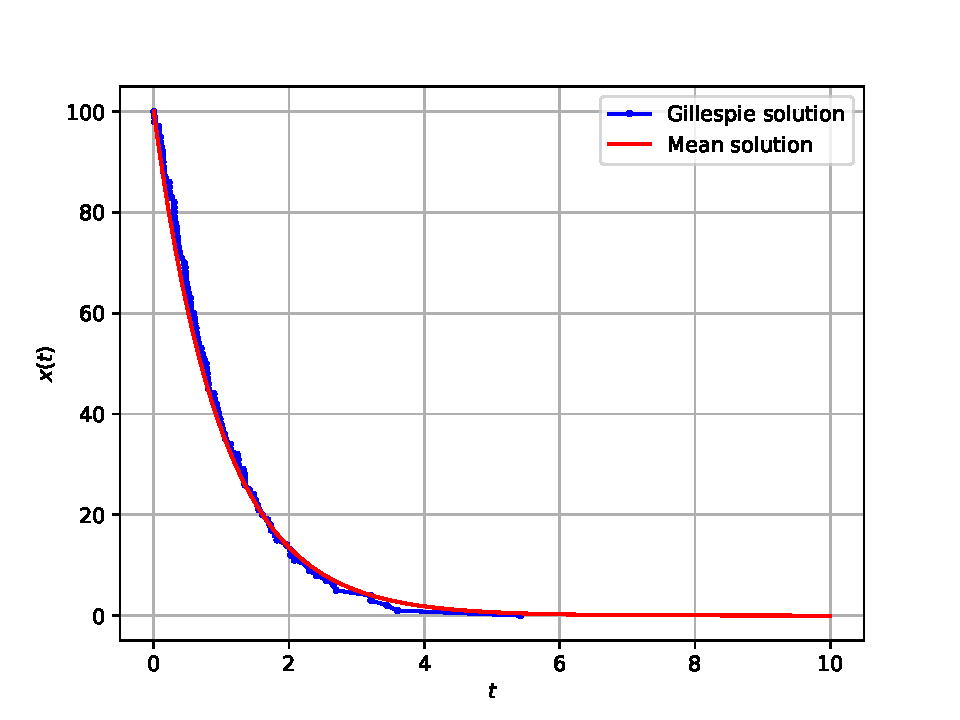
\includegraphics[width=0.75\textwidth]{../pictures/lab7_eq_1.pdf}
  \caption{Решения уравнения распада, полученные различными методами}
  \label{fig:1d_decay}
\end{figure}

\section{Решение системы уравнений}
Во второй части работы следующая система была смоделирована как случайный процесс:
\begin{displaymath}
  \left\{
  \begin{array}{lr}
    \dot x = 2 x_2 - 2x^2\\
    \dot x_2 = x^2 - x_2
  \end{array}
\right.
\end{displaymath}
Начальные условия: \(x(0)=100,\;x_2(0)=0\). Также данная система была решена методом Рунге-Кутты 4го порядка.
Все решения получены для промежутка времени \(t\in[0,6]\). Детерминированное решение очень быстро приходит к одному
из расположенных на кривой \(x_2=x^2\) состояний равновесия, в то время как стохастическая реализация демонстрирует
колебания относительно состояния равновесия.

\begin{figure}[H]
  \center
  \subfloat[]{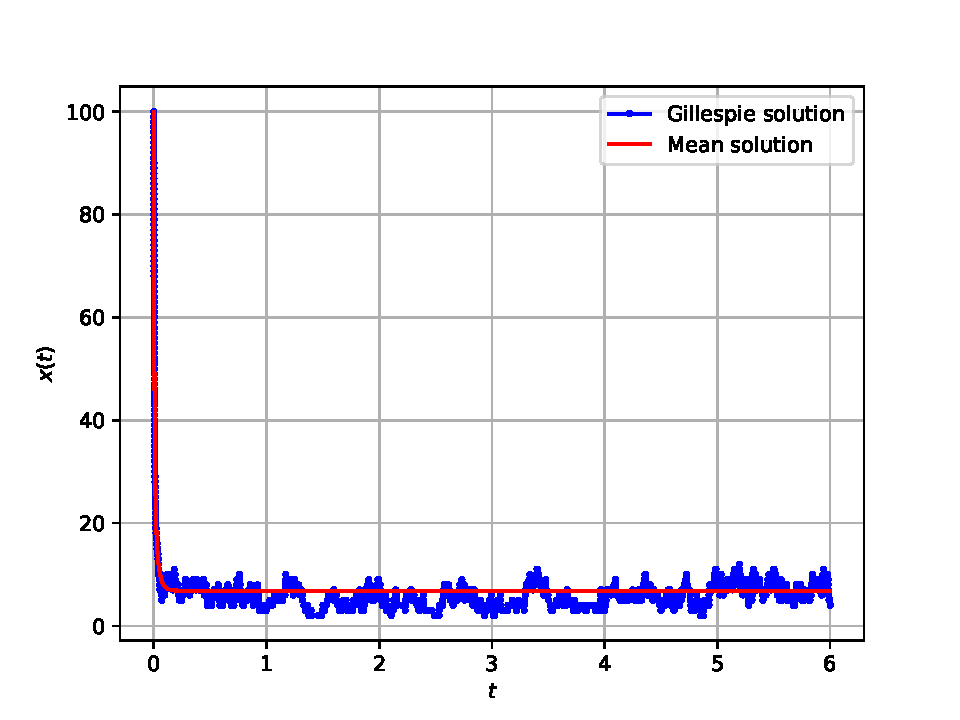
\includegraphics[width=0.6\textwidth]{../pictures/lab7_eq_2_1.pdf}\label{fig:2d_1}}
  \subfloat[]{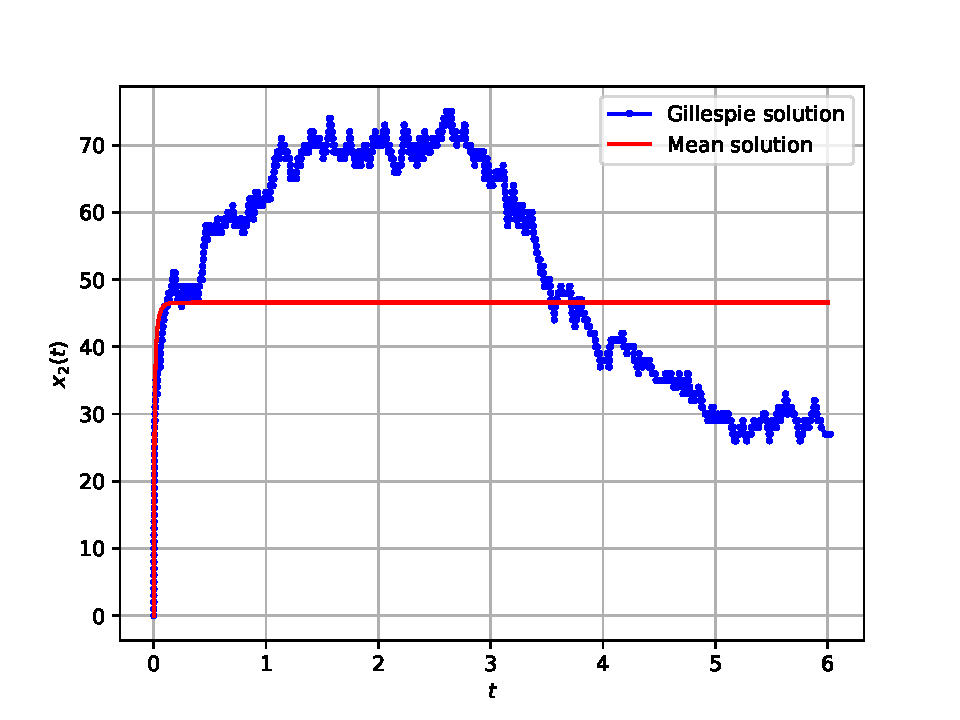
\includegraphics[width=0.6\textwidth]{../pictures/lab7_eq_2_2.pdf}\label{fig:2d_2}}
  \caption{Решения системы уравнений}
\end{figure}

\section{Исходный код}
\lstinputlisting[language=Python, numbers=left]{../scripts/lab7.py}

\end{document}
